\chapter{Proof-of-concept implementatie met OpenMetadata}
\label{ch:poc-implementatie}

\section{Doel en positionering van de proof-of-concept}

Zoals beschreven in Hoofdstuk~\ref{ch:contextanalyse} ontstaat de grootste zichtbaarheids\-kloof in de huidige lineageketen bij VLAIO tussen de platinum-datasets in de Databricks-lake\-house omgeving en de daarop gebaseerde Power BI-rapporten. Deze PoC heeft als doel om die laatste stap expliciet te maken in OpenMetadata, door Power BI-metadata systematisch te koppelen aan bestaande tabellen in de vorm van OpenMetadata entiteiten en daaruit een bruikbare lineageketen op te bouwen.\\

Dit hoofdstuk beschrijft ten eerste de technische architectuur en de gebruikte metadata bronnen. Vervolgens wordt de mappingstrategie voor het koppelen van Power BI aan platinum-datasets toegelicht, gevolgd door een overzicht van de end-to-end-implementatie voor het genereren van de lineage in OpenMetadata. Tot slot worden de automatisatie, de belangrijkste beperkingen van de PoC en de visuele resultaten besproken. Hoewel de illustratieve voorbeelden in dit hoofdstuk voornamelijk focussen op de Steunster en Krissteunster-rapporten\footnote{Steunster en Krissteunster zijn datasetmodellen in de vorm van een sterschema die een overzicht geven van alle steun die een onderneming bij VLAIO vraagt, krijgt en geweigerd wordt, met daarbij relevante informatie over maatregelen en dossierkenmerken. Krissteunster is een uitbreiding van Steunster.}, is de onderliggende aanpak bewust generiek opgezet en uitgevoerd voor alle rapporten.\\

De PoC is uitgewerkt als een reeks herbruikbare Databricks-notebooks in een Git-repository binnen de Databricks-werkruimte. De kernfunctionaliteit bestaat uit:
\begin{itemize}
	\item het opzetten en testen van een verbinding met de OpenMetadata-client
	\item het inlezen en verwerken van metadata over Power BI-datasets en -rapporten via SQL-query's op de Databricks-tabellen
	\item het genereren van mappings tussen Power BI-datasetnamen en onder\-liggen\-de platinum-datasets op basis van een hulpscript
	\item het aanmaken van dash\-board-en\-ti\-tei\-ten in OpenMetadata voor Power BI-rap\-por\-ten
	\item het leggen van lineage-edges tussen platinum-tabellen en de aangemaakte dash\-board-en\-ti\-tei\-ten
\end{itemize}

Alle implementatiestappen zijn opgezet met zodat ze herbruikbaar zijn wanneer er nieuwe rapporten of datasets worden toegevoegd. Lokale configuratie (JWT-token\footnote{Een JWT-token of JSON Web Token)is digitale sleutel die wordt gebruikt om een gebruiker of systeem te authenticeren bij een API.}, pad naar metadatafiles) worden daarom gescheiden gehouden van de generieke logica voor mapping en lineage-opbouw.\\

\section{Technische omgeving en architectuur}

Hoewel OpenMetadata standaard een Power BI-connector aanbiedt voor het automatisch aanmaken van dashboards en lineage,\footnote{Zie de officiële documentatie van OpenMetadata voor de Power BI-connector: \url{https://docs.open-metadata.org/v1.12.x/connectors/dashboard/powerbi}.} kon deze in de VLAIO-context niet gebruikt worden. De nodige rechten en rechtstreekse toegang tot de Power BI REST API ontbreken op het niveau waarop OpenMetadata draait, waardoor een directe connectorconfiguratie niet haalbaar was. In theorie zou lineage ook volledig manueel kunnen worden opgebouwd via de gebruikersinterface, maar voor het grote aantal datasets en rapporten zou dit een zeer arbeidsintensieve en foutgevoelige aanpak zijn.\\

Om die redenen is in deze PoC gekozen voor een alternatieve aanpak, waarbij Power BI-metadata uit Databricks wordt ingelezen en vervolgens via de OpenMetadata SDK programmatisch wordt omgezet naar dashboard-entiteiten en li\-ne\-age-ed\-ges. Het is hierbij belangrijk op te merken dat zo'n aangemaakte dashboard-entiteit op OpenMetadata slechts een abstracte representatie is van een echt Power BI-rapport en geen fysiek of interactief dashboard op zich. De oorspronkelijke rapport-URL wordt wel meegegeven als \texttt{sourceUrl}, zodat de gebruiker vanuit OpenMetadata snel kan doorklikken naar werkelijke rapport. Wanneer in het vervolg van dit hoofdstuk dus gesproken wordt over het `aanmaken of verwijderen van dashboards', wordt daarmee dan ook expliciet de dash\-board-en\-ti\-teit binnen het OpenMetadata bedoeld.\\

Initieel werd lokaal gewerkt om de Api van OpenMetadata te testen en een eerste werkende POC op te zetten. Voor de uiteindelijke realisatie en automatisering werd de implementatie overgezet naar de Data\-bricks-omgeving, waarbij gebruik kon gemaakt worden van een cluster. Zo een cluster is een rekenomgeving in Databricks dat bestaat uit één of meerdere virtuele machines. Deze leveren dan de rekencapaciteit om notebooks en pipelines uit te voeren. Hierop zijn de nodige Python-packages geïnstalleerd, waardoor ze beschikbaar zijn in alle notebooks zonder telkens een \texttt{pip install} uit te voeren. Bovendien maakt de integratie met Spark\footnote{Apache Spark is een open-source framework voor het snel verwerken van grote hoeveelheden data.} het mogelijk om binnen notebooks rechtstreeks de benodigde data en metadata op te vragen.\\

Voor de uiteindelijke lineage POC wordt gebruik gemaakt van de OpenMetadata-omgeving binnen VLAIO. De verbinding hiermee gebeurt via de publieke API endpoint \texttt{https://omd.data-services-dev.vlaio.be/api}, met een JWT-token dat via een lokale \texttt{.env}-configuratie wordt ingelezen. Op basis daarvan wordt een Open\-Me\-ta\-da\-ta-client opgebouwd, die in de rest van de notebooks wordt hergebruikt om entiteiten op te vragen en te creëren. Deze client is gebaseerd op de Python SDK\footnote{Een Software Development Kit is een verzameling voorgebouwde functies en klassen die het mogelijk maken om met een platform te communiceren in code.} van OpenMetadata, die de interactie met de API vereenvoudigt. Hierdoor kunnen voorgebouwde functies worden gebruikt en is het niet nodig om zelf HTTP-verzoeken samen te stellen. Zoals reeds vermeld in Hoofdstuk~\ref{ch:contextanalyse} was de Databricks service al geconnecteerd en de datasets en tabellen dus beschikbaar. Om deze tabellen aan rapporten te kunnen koppelen, moeten de Power BI-rapporten ook eerst beschikbaar zijn in OpenMetadata. Daarvoor is een Power BI-service nodig. In dit geval is dat \texttt{VLAIO_POWERBI_TEST}. Deze service was al aangemaakt in OpenMetadata. Indien dat niet het geval zou zijn, kan een nieuwe service eenvoudig toevoegen via de gebruikersinterface of met de Python-SDK. Zonder een gekoppelde service is het immers niet mogelijk om Power BI-gerelateerde entiteiten aan te maken op OpenMetadata.\\

De implementatie is opgebouwd als twee Databricks-notebooks die samen de volledige flow van de lineage-objecten beheren:
\begin{itemize}
	\item \texttt{detect\_changes\_and\_apply\_lineage}: de hoofdnotebook die de volledige end-to-end-flow uitvoert, van het ophalen van Power BI-metadata uit Databricks-tabellen tot het aanmaken van dashboards en lineage-edges in OpenMetadata
	\item \texttt{Delete\_OpenMetadata\_lineage}: een opschoningsnotebook waarmee alle eerder aangemaakte dashboards en lineage-edges efficiënt en parallel verwijderd kunnen worden
\end{itemize}

Naast de twee hoofdnotebooks bevat de repository een aantal scripts en notebooks die tijdens de ontwikkeling gebruikt werden om de interactie met de API van OpenMetadata gefaseerd te verkennen en te testen. Deze scripts vormen geen onderdeel van de uiteindelijke end-to-end-flow, maar hebben een belangrijke rol gespeeld in het opbouwen en testen van de kernfunctionaliteit:
\begin{itemize}
	\item \texttt{client\_config.py}: hulpfunctie om de OpenMetadata-client in te stellen en de verbinding te testen
	\item \texttt{create\_dashboard.py}: voorbeeldscript dat laat zien hoe een dash\-board-en\-ti\-teit aangemaakt kan worden via de SDK
	\item \texttt{add\_lineage\_edge.py}: voorbeeldscript om een lineage-edge tussen twee bestaande entiteiten toe te voegen
	\item \texttt{get\_table\_by\_id.py}: script om een tabel op te zoeken op basis van id of fully-qualified name (FQN) en het resultaat van de API-call te inspecteren
	\item \texttt{Platinum\_en\_PowerBI\_Datasets.py}: notebook voor het ophalen en exporteren van metadata uit OpenMetadata en Databricks, waaronder platinum datasets, Power BI-datasets en bijhorende rapportinformatie
	\item \texttt{Create\_OpenMetadata\_lineage.py}: eerste volledige eenvoudige versie van de lineageflow, waarin dashboards worden aangemaakt en lineage-relaties worden gelegd op basis van CSV- en YAML-mappings
\end{itemize}

Tokens en andere geheimen worden niet in de notebooks zelf opgeslagen, maar via een lokale \texttt{.env}-configuratie ingelezen. Zo blijft de code zelf herbruikbaar, zonder gevoelige informatie prijs te geven. Naast de JWT-token worden ook de OpenMetadata API-URL (\texttt{OM\_HOST}), de dashboardservice (\texttt{DASHBOARD\_SERVICE}) en de database-identifiers uit dit \texttt{.env}-bestand gelezen. De SQL-tabelnamen (\texttt{SILVER\_DATASET\_TABLE}, \texttt{SILVER\_REPORT\_TABLE}) zijn als variabelen centraal bovenaan de notebook gedefinieerd. Hierdoor moeten bij een eventuele productie-uitrol enkel deze configuratiewaarden aangepast worden, zonder wijzigingen aan de logica zelf.\\

\section{Datasets en metadata-bronnen}

Voor de realisatie van de PoC worden twee typen metadata gecombineerd, die binnen de Databricks- en OpenMetadata-omgeving uit de volgende bronnen worden onttrokken:

\begin{itemize}
	\item \textbf{Power BI-metadata:} Dit betreft metadatadumps die afkomstig zijn uit de Power BI REST API en als tabellen beschikbaar zijn in de silver-laag van Databricks. Deze worden binnen de pipeline rechtstreeks via Spark uitgelezen uit:
	\begin{itemize}
		\item \texttt{ccdata_dev.silver.powerbirestapi_report}: bevat rapportgegevens, waaronder de rapportnaam, web-URL, het unieke rapport-ID en het gekoppelde dataset-ID.
		\item \texttt{ccdata_dev.silver.powerbirestapi_dataset}: bevat datasetgegevens, zoals de datasetnaam en het bijbehorende dataset-ID.
	\end{itemize}
	\item \textbf{Platinum-datasets:} Een overzicht van de beschikbare platinum datasets binnen de Databricks-lakehouse-omgeving. Aangezien deze reeds in OpenMetadata aanwezig zijn, worden ze opgehaald via de OpenMetadata-API met de functie \texttt{DatabaseSchemas.list_all}, voorzien van een filter op de platinum-laag.
\end{itemize}

De bedoeling is dus om alle Power BI-datasets te koppelen aan de bijhorende platinum datasets. Als deze mapping vastligt kan nadien correcte lineage toegevoegd worden. In de eerste versie van de PoC werd gewerkt met CSV-exports uit Databricks als input voor de mapping en lineage-scripts. In de huidige implementatie worden de Power BI-metadata rechtstreeks via SQL uit de Databricks-tabellen opgehaald, waardoor alles reproduceerbaar is en de pipeline volledig geautomatiseerd kan draaien.\\

Binnen OpenMetadata was de platinum laag al aanwezig door de koppeling met Databricks. De PoC voegt hieraan een extra laag toe. Power BI-dashboards en lineage-edges die laten zien welke platinum-tabellen de belangrijkste bron vormen voor een bepaald rapport. Om de lineage overzichtelijk en functioneel te houden, wordt bij datasets die een sterschema volgen, specifiek gekozen voor de fact tabel(len). Deze vormen het centrum van een schema met daarin de belangrijkste info, terwijl dimensietabellen enkel context bieden. Bij overige datasets wordt op dezelfde manier gefocust op de voornaamste brontabel(len). Een alternatief was om een rapport-entiteit met alle tabellen van de bijhorende dataset te verbinden, maar dit zou zorgen veel meer verbindingen, waardoor de voorstelling van de lineage voor de gebruikers zeer onoverzichtelijke zou worden.

\paragraph{Afleiding van Power BI-rapporten uit Databricks.}

Omdat OpenMetadata in de huidige VLAIO-omgeving niet rechtstreeks kan verbinden met de Power BI REST API, werd gebruikgemaakt van de afgeleide Power BI-metadata die reeds onder vele tabellen in Databricks beschikbaar is. Deze tabellen waren niet vooraf gedocumenteerd voor het doel van lineage, waardoor eerst manueel onderzocht moest worden welke data hieruit gebruikt kon worden om een overzicht van rapporten en bijbehorende datasets op te bouwen. Na het verkennen van de relevante tabellen werd onderstaande query opgesteld als basis om alle rapporten met hun datasetnaam te extraheren. Hiermee was de nodige metadata aanwezig om de dash\-board-en\-ti\-tei\-ten aan te maken en deze nadien te koppelen aan de bron tabel uit de platinum laag.\\

Deze brontabellen bevatten historische snapshots volgens het \textit{Slowly Changing Dimension type 2} (SCD) Type 2\footnote{Bij SCD Type 2 wordt een nieuwe record aangemaakt telkens een gegeven wijzigt, in plaats van de bestaande record te overschrijven. Zo blijft de volledige historiek bewaard.}, waarbij elke record wordt beheerd met de kolommen \texttt{RawDataStartDatum} en \texttt{RawDataEindDatum}. Om dus een actueel overzicht op te bouwen, is het belangrijk om uitsluitend de meest recente snapshot van elk rapport te selecteren. Hiervoor wordt gebruikgemaakt van het Boolean-veld \texttt{RawDataIsCurrent}. De gebruikte query ziet er uit als volgt:

\begin{lstlisting}[language=SQL, caption={Query om de meest recente Power BI-metadata te selecteren}, label={lst:powerbirest-query}]
	SELECT r.RapportNaam, 
		   r.WebUrl, 
		   d.DatasetNaam, 
		   r.RapportID, 
		   r.DatasetID
	FROM ccdata_dev.silver.powerbirestapi_report r
	JOIN ccdata_dev.silver.powerbirestapi_dataset d
	ON r.DatasetID = d.DatasetID
	WHERE r.RawDataIsCurrent = true AND d.RawDataIsCurrent = true
	AND d.RawDataIsCurrent = true
	ORDER BY d.DatasetNaam, r.RapportNaam;
\end{lstlisting}

In de implementatie worden de tabelnamen niet hardgecodeerd maar via f-strings met de variabelen \texttt{SILVER\_REPORT\_TABLE} en \texttt{SILVER\_DATASET\_TABLE} ingevuld, zodat de query ongewijzigd werkt in zowel de dev als productie-omgeving.\\

De kolom \texttt{RapportOmschrijving} werd hier bewust niet gebruikt, omdat deze in de praktijk vrijwel altijd leeg bleek en dus weinig meerwaarde had voor de PoC. Indien deze ingevuld is kan deze ook meegegeven worden aan OpenMetadata. In de huidige implementatie wordt deze query rechtstreeks vanuit de notebook uitgevoerd met spark, waardoor de resultaten onmiddellijk beschikbaar zijn voor verdere verwerking. De resultaten worden vervolgens weggeschreven naar een CSV-bestand als tussenstap, zodat de daaropvolgende stappen op de cluster kunnen draaien zonder opnieuw de SQL-query uit te voeren.\\

In de oorspronkelijke versie van de query werd gefilterd op \texttt{DatasetNaam = 'VLAIO Steunster'} om bij de eerste experimenten te focussen op één concrete dataset. In de huidige implementatie is deze filter verwijderd. Alle rapporten worden opgehaald en vervolgens gefilterd op basis van de YAML-mappings, zodat de pipeline generiek werkt voor alle mappeerbare datasets.\\

\section{Mapping van Power BI-datasets naar platinum-datasets}

\subsection{Algemene mappingstrategie}

In de beschikbare metadata is per rapport een veld \texttt{Datasetnaam} aanwezig, naast een lijst van alle platinum-datasets. Om lineage te kunnen opbouwen, moet er een koppeling worden gemaakt tussen deze twee. Dit brengt echter enkele uitdagingen met zich mee. Niet elk rapport is gebaseerd op een platinum-dataset, zo steunen sommige bijvoorbeeld op Excel-bestanden of andere bronnen. Bovendien komen de veldwaarden zelden exact overeen met de datasetnamen, waardoor deze niet direct kunnen gebruikt worden om lineage te creëren. De kern van de PoC is dus een generieke mappinglaag, die het veld \texttt{Datasetnaam} gebruikt om voor elk rapport een koppeling te maken met de onderliggende platinum-dataset. Deze mapping gebeurt niet via handmatig ingevulde lijsten, maar via een set heuristieken die de namen in beide domeinen op verschillende manieren met elkaar vergelijkt. De implementatie maakt gebruik van het volgende script voor het genereren van de mappings:
\begin{itemize}
	\item \texttt{\_build\_mapping.py}: dit script bouwt de mapping tussen de volledige lijst van Power BI-datasets en de platinum-datasets. Dit script genereert twee verschillende outputs:
	\begin{itemize}
		\item \textbf{Confirmed mapping:} bevat de meest betrouwbare, automatisch goedgekeurde matches op basis van de gedefinieerde logica.
		\item \textbf{Review mapping:} verzamelt alle datasets en rapporten die niet gematcht konden worden, zodat deze handmatig gecontroleerd of aangevuld kunnen worden.
	\end{itemize}
\end{itemize}

In de context van deze bachelorproef wordt deze mappinggenerator vooral gebruikt als hulpmiddel om een eerste, zo volledig mogelijke basisversie op te bouwen. Daarnaast zou door het grote aantal datasets een volledige manuele mapping namelijk zeer veel tijd innemen. Bovendien maakt dit de mapping ook reproduceerbaar. 
Hoewel de gegenereerde output de basis vormt voor de uiteindelijke lineage-pipeline, maakt dit mapping script zelf geen deel uit van de uiteindelijke end-to-end workflow. Het diende vooral om aan te tonen hoe een naamgebaseerde aanpak kan helpen om snel een betrouwbaar startpunt te creëren.\\

\subsection{Naamgebaseerde mapping en outputstructuur}

De mapping scripts standaardiseren de namen eerst door hoofdletters, speciale tekens en afwijkende schrijfwijzen weg te werken. Daarna worden verschillende regels toegepast om mogelijke koppelingen te beoordelen. Hierbij worden verschillende naamgebaseerde vergelijkingsstrategieën gecombineerd, zoals exacte matching, deelstringvergelijkingen, fuzzy matching\footnote{Fuzzy matching vindt overeenkomsten tussen teksten die niet exact gelijk zijn, maar sterk op elkaar lijken.} en token-gebaseerde vergelijkingen\footnote{Bij token-gebaseerde vergelijking worden namen opgesplitst in afzonderlijke woorden of delen, waarna die tokens apart worden vergeleken.}. Deze genereren dan per gevonden match een score en op basis daarvan worden de potentiële koppelingen automatisch geclassificeerd naar betrouwbaarheid. De resultaten worden vervolgens weggeschreven naar aparte CSV-bestanden, zodat duidelijke matches rechtstreeks gebruikt kunnen worden en twijfelgevallen apart beschikbaar blijven voor een eventuele manuele controle.\\

De mapping-output ondersteunt ook multi-mapping. Elke Power BI-dataset kan, indien nodig, aan meerdere platinum-datasets gekoppeld worden. De kolom \texttt{platinum\_datasets} bevat dan een lijst van kandidaten, en \texttt{match\_count} geeft het aantal matches weer. Dergelijke situaties krijgen een aparte status namelijk \texttt{confirmed\_multi}, zodat downstream-logica hiermee rekening kan houden. Een voorbeeld hiervan is \texttt{Krissteunster-Steunster Composite model} zoals te zien op tabel \ref{tab:mapping-confirmed}. Dit is een samenstelling van twee platinum datasets, dat moet gemapt worden naar zowel Steunster als Krissteunster.\\

In de meest recente run verwerkte de mappinggenerator 418 Power BI-datasets, waarvan 117 als \texttt{confirmed} en 4 als \texttt{confirmed\_multi} werden geclassificeerd. De overige 297 datasets bleven \texttt{unmatched}. Dat is niet noodzakelijk een tekortkoming van de mappinglogica. Niet elke Power BI dataset heeft een tegenhanger in de platinum-laag. Bronnen zoals lokale Excel-bestanden of SharePoint-lijsten bestaan simpelweg niet in Databricks en kunnen dus niet gemapt worden. Deze ongematchte gevallen vragen wel een manuele controle om een onderscheid te maken tussen terecht niet-koppelbare datasets en uitzonderingen, die alsnog handmatig aan de YAML-configuratie toegevoegd moeten worden.\\

Die manuele controlelaag komt voort uit de manier waarop Power BI metadata wordt gegenereerd. De export van datasetnamen uit de REST API toont dat deze vaak zijn gebaseerd op de bestandsnamen van de lokale \texttt{.pbix}-bestanden. Namen zoals \textit{``model coosy PRD  14-01-2026''} of \textit{``Bedrijventerreinenster\_0126''} bevatten handmatige versienummers, datumstempels of andere toevoegingen die sterk afwijken van de naamgeving in de platinum-laag. Bij bestandsnamen die inhoudelijk totaal niet meer lijken op de brontabel, is een automatische koppeling simpelweg onmogelijk.\\

\paragraph{Voorbeeld van mapping-output (CSV).}

Onderstaand fragment illustreert hoe de output van het mappingscript eruitziet in \texttt{PowerBI\_to\_Platinum\_mapping\_confirmed.csv}. Tabel \ref{tab:mapping-confirmed} toont dat de Power BI-dataset niet noodzakelijk exact overeen moet komen met de naam van de bijhorende platinum-dataset, om toch een correcte koppeling te krijgen (zie bijvoorbeeld \textit{Heropstartlening}). Vooraleer deze mappings worden omgezet naar de YAML-configuratie die effectief gebruikt wordt voor het aanmaken van lineage, moeten ze uiteraard manueel nagekeken worden.\\

\begin{table}[h]
	\centering
	\small
	\begingroup
	\renewcommand{\arraystretch}{2}
	\begin{tabularx}{\textwidth}{>{\raggedright\arraybackslash}X
			>{\raggedright\arraybackslash}X
			>{\centering\arraybackslash}p{1.4cm}
			>{\centering\arraybackslash}p{1.8cm}
			>{\raggedright\arraybackslash}p{2.6cm}}
		\hline
		\textbf{Power BI-dataset} & \textbf{Platinum-dataset(s)} & \textbf{Aantal} & \textbf{Score} & \textbf{Status} \\
		\hline
		Bedrijventerreinenster & bedrijventerreinenster & 1 & 1.000 & confirmed \\
		Contactenster & contactenster & 1 & 1.000 & confirmed \\
		KRISsteunster & krissteunster & 1 & 1.000 & confirmed \\
		Krissteunster--Steunster Composite model & krissteunster;steunster & 2 & 0.990 & confirmed\_multi \\
		Corona -- Heropstartlening & r\_coronaheropstartlening & 1 & 0.980 & confirmed \\
		\hline
	\end{tabularx}
	\endgroup
	\caption{Verkort fragment uit \texttt{PowerBI\_to\_Platinum\_mapping\_confirmed.csv}.}
	\label{tab:mapping-confirmed}
\end{table}

\paragraph{Voorbeeld van Power BI-datasetmappings (YAML).}

Na de handmatige controle en eventuele verbeteringen worden de definitieve koppelingen met het script \texttt{fill\_powerbi\_yaml\_from\_mappings.py} omgezet naar een configuratie in YAML. Er is bewust gekozen voor een YAML-structuur als centrale configuratielaag vanwege de goede leesbaarheid en de flexibiliteit die het biedt tijdens de ontwikkelfase. Het formaat maakt het voor zowel ontwikkelaars als niet-technische stakeholders eenvoudig om bestaande mappings in te zien, snel handmatige correcties door te voeren of nieuwe uitzonderingen toe te voegen zonder de overhead van bijvoorbeeld een database-migratie. Daarnaast biedt YAML de nodige granulariteit om, naast generieke dataset-mappings, ook specifiekere verfijningen toe te voegen.

Dat laatste is bijvoorbeeld het geval in het onderstaande fragment voor \texttt{Epplus betalingen}. Deze Power BI-dataset wordt enerzijds nog steeds logisch gekoppeld aan de platinum-dataset \texttt{r\_epplus}, maar anderzijds wordt ook expliciet de tabel \texttt{epp\_betalingen} meegegeven. Hierdoor verwijst de lineage in dit geval niet naar alle fact- of brontabellen binnen \texttt{r\_epplus}, maar enkel naar de concrete tabel waarvoor voldoende zekerheid bestaat dat ze effectief in het rapport gebruikt wordt. De YAML-structuur laat dus zowel generieke mappings op datasetniveau als meer precieze mappings op tabelniveau toe, afhankelijk van de hoeveelheid beschikbare metadata.

\begin{lstlisting}[language=YAML, caption={Fragment uit PowerBI\_Dataset\_Mappings.yml}, label={lst:yaml-pbi}]
	- PBIDataset: VLAIO Steunster
	  target_datasets:
		- steunster
	
	- PBIDataset: KRISsteunster
	  target_datasets:
		- krissteunster
	
	- PBIDataset: Krissteunster-Steunster Composite model
	  target_datasets:
		- krissteunster
		- steunster
	
	- PBIDataset: Dataset PBIDatasetsMetRollen
	  target_datasets:
		- r_pbidatasetsmetrollen
		
	- PBIDataset: Epplus betalingen
	  target_datasets:
		- r_epplus
	  target_tables:
		- lz02-d-dbw-ccdata-main.platinum_dev.r_epplus.epp_betalingen
	
\end{lstlisting}

\paragraph{Voorbeeld van platinum-datasetmappings (YAML).}

Aangezien lineage in OpenMetadata volgens de gangbare aanpak op tabelniveau wordt vastgelegd, volstaat het niet om enkel een koppeling te maken tussen een Power BI-dataset en een logische platinum-dataset. Daarom werd aanvullend een manuele mapping opgesteld waarin per platinum-dataset wordt vastgelegd welke concrete tabellen als meest relevante bron voor de lineage beschouwd worden. Zoals eerder vermeld wordt daarbij in de eerste plaats gekozen voor facttabellen wanneer die beschikbaar zijn, en anders voor de belangrijkste tabellen binnen de betrokken dataset.\\

In \texttt{Platinum\_Dataset\_Mappings.yml} worden de logische platinum-datasets verder vertaald naar een of meerdere specifieke tabellen. Om de herbruikbaarheid en omgevingsonafhankelijkheid van de pipeline te garanderen, worden in deze YAML-configuratie enkel de schema en tabelnamen (zoals \texttt{krissteunster.f\_steun}) opgenomen, in plaats van volledige, hardgecodeerde \textit{Fully Qualified Names} (FQN's).\\

Verwijzingen naar omgevingsspecifieke waarden, zoals databasenamen of de eerste delen van een FQN  (\texttt{lz02-d-dbw-ccdata-main.platinum\_dev}) worden als omgevingsvariabelen ingesteld. De scriptlogica voegt deze omgevingsvariabelen vervolgens samen met de tabelnaam uit de YAML om de uiteindelijke FQN op te bouwen. Zo kunnen deze gewijzigd worden buiten de logica zelf. Deze resulterende FQN is noodzakelijk om de tabelentiteiten uniek te kunnen identificeren en correct te koppelen binnen OpenMetadata. Deze aanpak zorgt ervoor dat de mapping configuratie ongewijzigd kan functioneren in verschillende omgevingen, zoals bijvoorbeeld dev of productie.\\

De YAML-opzet blijft hierdoor bovendien makkelijk uitbreidbaar en aanpasbaar. Nieuwe datasets of bijkomende tabellen kunnen zonder aanpassing van de code eenvoudig worden toegevoegd, terwijl bestaande mappings ook verfijnd kunnen worden wanneer extra domeinkennis beschikbaar wordt of de datamodellen wijzigen.\\

\begin{lstlisting}[language=YAML, caption={Fragment uit Platinum\_Dataset\_Mappings.yml}, label={lst:yaml-platinum}]
	- dataset: krissteunster
	target_tables:
	- krissteunster.f_steun
	- krissteunster.f_steunster
	- krissteunster.f_steunster_toegevoegdewaarde
	
	- dataset: steunster
	target_tables:
	- steunster.f_steun
\end{lstlisting}


\section{Dashboards en lineage in OpenMetadata}

\subsection{End-to-end-flow}

De lineage-pipeline verloopt in meerdere stappen, van het ophalen van Power BI-metadata in Databricks tot zichtbare lineage op OpenMetadata. Deze volledige flow wordt uitgevoerd vanuit de notebook \texttt{detect\_changes\_and\_apply\_lineage} en bestaat uit:
\begin{enumerate}
	\item Ophalen van alle Power BI-rapporten en bijhorende datasetnamen via een SQL-query op de Databricks-tabellen (Spark), gefilterd op \texttt{RawDataIsCurrent = true}.
	\item Exporteren van de queryresultaten naar een CSV-bestand als tussenstap.
	\item Opzoeken van de YAML-mappings en filteren op rapporten waarvoor een geldige mapping bestaat naar minstens een platinum-tabel. Ongemapte datasets worden automatisch weggeschreven naar \texttt{unmapped\_datasets.csv}.
	\item Een prefetch van alle bestaande dashboards in OpenMetadata en categorisatie van elk rapport in drie paden: nieuw (aanmaken), te updaten (naam gewijzigd), of over te slaan (ongewijzigd).
	\item Parallel aanmaken of updaten van dash\-board-en\-ti\-tei\-ten in OpenMetadata voor de gecategoriseerde rapporten.
	\item Parallel aanmaken van lineage-edges van de relevante platinum-tabellen naar de aangemaakte dashboards.
	\item Wegschrijven van gedetailleerde logging naar een logbestand.
\end{enumerate}

In de Power BI REST API-tabellen zijn in totaal 4194 rapportrijen aanwezig. Dit totaalcijfer bevat echter een groot aantal verouderde snapshots van dezelfde rapporten. Door in de SQL-query specifiek te filteren op de meest recente status, worden enkel de 1165 unieke, actuele rapporten opgehaald. Hiervan hebben 464 rapporten een geldige mapping in de YAML-configuratie, die effectief verwijst naar minstens één bestaande platinum-tabel in OpenMetadata. Enkel deze rapporten worden vervolgens doorgestuurd naar de dashboardcreatie- en lineage-stappen. Deze filtering voorkomt dat er onnodige of onvolledige entiteiten in OpenMetadata worden aangemaakt.\\

De focus ligt op lineage op tabelniveau: voor elk rapport wordt minstens een lineage-edge gelegd vanaf de belangrijkste platinum-tabel naar het dashboard, aangevuld met extra edges bij samengestelde datasets. Op die manier ontstaat er een visueel traceerbare keten van bronsystemen via medallion-lagen (bronze, silver, platinum) tot en met de rapportages.\\

\subsection{Belangrijkste notebook-code}

Onderstaande paragrafen beschrijven de kernlogica uit de notebook. Ter ondersteuning zijn enkele belangrijke codefragmenten opgenomen. Voor de leesbaarheid zijn bijkomende zaken als uitgebreide imports, tussentijdse logging, robuuste foutafhandeling en hulpfuncties weggelaten.

\paragraph{OpenMetadata-connectie}

Dit codefragment initialiseert de verbinding met OpenMetadata en zorgt ervoor dat de notebook geauthenticeerd kan communiceren met OpenMetadata. Eerst wordt een JWT-token uit de omgevingsvariabelen geladen, waarna de connectieparameters voor de OpenMetadata-server en de dashboardservice worden ingesteld. Deze parameters worden uitgelezen uit het \texttt{environment} bestand en zijn niet hardgecodeerd. Dit zorgt ervoor dat het makkelijk herbruikbaar is in de productieomgeving. Bij een eventuele uitrol moeten enkel de omgevinsgvariabelen in \texttt(.env) aangepast worden en niets in de code zelf. Tot slot wordt gecontroleerd of de verbinding succesvol tot stand komt, zodat de volgende stappen enkel worden uitgevoerd wanneer de metadata-omgeving bereikbaar is. Hier worden ook de omgevingsvariabelen voor de FQN ingesteld.\\

\begin{lstlisting}[language=python, caption={OpenMetadata clientconnectie}, label={lst:om-connectie}]
# (hier worden alle imports en omgevingsvariabelen geladen)
jwt = os.getenv("JWT_SECRET")

# Hier wordt de OpenMetadata-host en de dashboardservice ingesteld
OM_HOST = os.getenv("OM_HOST", "https://omd.data-services-dev.vlaio.be/api")
DASHBOARD_SERVICE = os.getenv("DASHBOARD_SERVICE", "VLAIO_POWERBI_TEST")
OM_DATABASE_SCHEMA = os.getenv("OM_DATABASE_SCHEMA, "lz02-d-dbw-ccdata-main.platinum_dev")

# Serverconfiguratie voor de OpenMetadata-client
server_config = OpenMetadataConnection(
	hostPort=OM_HOST,
	authProvider="openmetadata",
	securityConfig=OpenMetadataJWTClientConfig(jwtToken=jwt),)

# initialisatie ometa-client en SDK-client
metadata = OpenMetadata(server_config)
configure(host=OM_HOST, jwt_token=jwt)
\end{lstlisting}

\paragraph{Batch-export van unieke rapporten}

In de huidige implementatie worden alle Power BI-rapporten in een enkele SQL-query opgehaald en naar een CSV-bestand geexporteerd. Dit geeft een lijst waarin de meest recente versie van elk uniek rapport één keer voorkomt. Technisch gezien is het geen probleem om hetzelfde dashboard meerdere keren via een API-aanroep naar OpenMetadata te sturen, maar door duplicaten vooraf weg te filteren worden onnodige API-aanroepen vermeden en blijft de verwerking efficiënt.\\

\paragraph{YAML-mapping en filtering op mappeerbare rapporten}

Na het ophalen van de raportdata worden de YAML-mappingbestanden ingelezen en wordt per rapport bepaald of een geldige koppeling naar minstens een platinum-tabel bestaat. Rapporten zonder geldige mapping worden uitgefilterd en komen niet in aanmerking voor verdere verwerking. De resolverfunctie gebruikt hierbij volgende prioriteitslogica: eerst worden direct opgegeven tabellen gezocht, en bij afwezigheid daarvan wordt de koppeling gelegd via de overkoepelende platinum-datasets.\\

Wanneer er in de toekomst nieuwe datasetnamen verschijnen in de Power BI REST API-tabel die nog niet in de YAML-configuratie zijn opgenomen, worden deze automatisch door de pipeline gedetecteerd en in het \texttt{unmapped_datasets.csv} bestand geplaatst. Dit zorgt ervoor dat de personen die de data beheren een actueel overzicht krijgen van nieuwe datasets. Hierdoor kunnen ze de mapping op een incrementele manier bijwerken. De volgende run zullen deze nieuwe mappings dan meegenomen worden en worden de bijhorende dashboards en lineage aangemaakt.

\begin{lstlisting}[language=python, caption={YAML-mapping en filtering}, label={lst:yaml-logica}]
POWERBI_MAPPING_PATH = "Mappings/PowerBI_Dataset_Mappings.yml"
PLATINUM_MAPPING_PATH = "Mappings/Platinum_Dataset_Mappings.yml"

# Dictionaries opbouwen uit YAML
power_bi_map = {}
for item in power_bi_yaml.get("datasets", []):
	pbi_name = str(item.get("PBIDataset", "")).strip()
	if not pbi_name:
		continue
	power_bi_map[normalize_key(pbi_name)] = {
		"target_tables": to_str_list(item.get("target_tables", [])),
		"target_datasets": to_str_list(item.get("target_datasets", [])),}

platinum_map = {}
# ... analoog als hiervoor, maar voor platinum-datasets

# Resolverfunctie met prioriteitslogica
def resolve_source_table_fqns(dataset_name: str) -> list[str]:
	mapping = power_bi_map.get(normalize_key(dataset_name))
	if not mapping:
		return []
	direct_tables = mapping.get("target_tables", [])
	if direct_tables:
		return unique_preserve_order(direct_tables)
	resolved = []
	for target_dataset in mapping.get("target_datasets", []):
		resolved.extend(platinum_map.get(
			normalize_key(target_dataset), []))
	return unique_preserve_order(resolved)

# Filter: enkel rapporten met geldige mapping behouden
df_mappable = df_unique[df_unique["DatasetNaam"].apply(
	lambda name: len(resolve_source_table_fqns(name)) > 0)]
\end{lstlisting}

\paragraph{Prefetch en parallelle dashboardcreatie}

Alvorens nieuwe dashboards aan te maken, worden alle bestaande dashboards in de Open\-Meta\-data-ser\-vice opgehaald en geïndexeerd op hun \texttt{name}-veld, dat overeenkomt met het \texttt{RapportID} (dit is een stabiele UUID). Hierbij wordt \texttt{RapportID} als \texttt{name} binnen OpenMetadata gebruikt en de leesbare \texttt{RapportNaam} als \texttt{displayName}, om worden naamconflicten vermeden. Zo worden twee rapporten met dezelfde naam maar een ander ID correct onderscheiden. Wanneer twee personen dus toevallig dezelfde rapportnaam kiezen, levert dit geen fout op en worden deze gezien als twee unieke rapporten.\\
Dit zorgt er ook voor dat de workflow herbruikbaar blijft, wanneer er nieuwe rapport-data binnenkomt in Databricks. Als de pipeline opnieuw wordt uitgevoerd, worden reeds bestaande dashboards herkend en overgeslagen zonder dubbels te creeren.\\

Op basis van deze prefetch wordt elk rapport gecategoriseerd in drie paden:
\begin{itemize}
	\item \textbf{Create}: het \texttt{RapportID} bestaat nog niet in OpenMetadata, dus er wordt een nieuw dashboard aangemaakt.
	\item \textbf{Update}: het \texttt{RapportID} bestaat al maar de \texttt{displayName} (= \texttt{RapportNaam}) is gewijzigd. het dashboard wordt bijgewerkt via \texttt{create\_or\_update}. Dit is nodig omdat rapporten in Power BI hernoemd kunnen worden terwijl het \texttt{RapportID} stabiel blijft (14 gevallen gevonden bij het testen).
	\item \textbf{Skip}: het \texttt{RapportID} bestaat al met identieke \texttt{displayName}, dus er moet niets gebeuren.
\end{itemize}

Daarna gebeurt de dashboardcreatie parallel via een \texttt{ThreadPoolExecutor}\footnote{Met een ThreadPoolExecutor kan je  meerdere taken gelijktijdig uitvoeren door ze te verdelen over een groep van parallelle threads.}, waarbij meerdere API-calls gelijktijdig worden verstuurd om de totale doorlooptijd te minimaliseren. Om de OpenMetadata-API niet te overbelasten, wordt het aantal parallelle werkers begrensd en wordt de HTTP-verbindingspool\footnote{Een HTTP-verbindingspool beheert een set herbruikbare verbindingen met een API. Door deze af te stemmen op het aantal threads wordt vermeden dat threads op elkaar moeten wachten voor een beschikbare verbinding.} afgestemd op het aantal actieve threads.\\

\begin{lstlisting}[language=python, caption={Prefetch en parallelle dashboardcreatie}, label={lst:parallel-dashboards}]
MAX_WORKERS = 10
POOL_SIZE = MAX_WORKERS + 5
	
# Prefetch: indexeer bestaande dashboards op name (= RapportID)
existing_by_report_id = {}
	for dashboard in Dashboards.list_all():
		d_name = str(getattr(dashboard, 'name', '')).strip().lower()
		if d_name:
			existing_by_report_id[d_name] = dashboard
	
# Categoriseer: nieuw / update / skip
new_reports, update_reports = [], []
for _, row in df_mappable.iterrows():
	rapport_id = row["RapportID"].strip().lower()
	existing = existing_by_report_id.get(rapport_id)
	if existing is None:
		new_reports.append(row)
	elif getattr(existing, 'displayName', '') != row["RapportNaam"]:
		update_reports.append(row)
	
# Verwerk elk rapport: name=RapportID (stabiel), displayName=RapportNaam
def process_report(row, mode='create'):
	request = CreateDashboardRequest(
		name=row["RapportID"], displayName=row["RapportNaam"],
		service=DASHBOARD_SERVICE, sourceUrl=row["WebUrl"],
		description=f"Dashboard voor dataset {row['DatasetNaam']}.",)
	if mode == 'create':
		dashboard = Dashboards.create(request)
	elif mode == 'update':
		dashboard = metadata.create_or_update(data=request, ...)
	return dashboard
	
with ThreadPoolExecutor(max_workers=MAX_WORKERS) as executor:
	futures = [executor.submit(process_report, row, 'create')
		for row in new_reports]
	futures += [executor.submit(process_report, row, 'update')
		for row in update_reports]
	for future in as_completed(futures):
		# ... resultaat ophalen en tellers bijwerken
\end{lstlisting}

\paragraph{Parallelle lineage-creatie}

Na het aanmaken van de dashboards worden de lineage-edges op dezelfde parallelle manier aangelegd. Per rapport worden de corresponderende brontabellen via de YAML-resolver bepaald en wordt voor elke combinatie van brontabel en dashboard een \texttt{AddLineageRequest} verstuurd. Het aanmaken van zowel de dashboards als de lineage bevat een ingebouwde retry-logica, zodat bij tijdelijke fouten automatisch opnieuw geprobeerd wordt. Deze logica is in de codevoorbeelden weggelaten om de leesbaarheid te behouden.\\

\begin{lstlisting}[language=python, caption={Parallelle lineage-creatie}, label={lst:lineage}]
seen_lineage_pairs = set()
lineage_created = 0
def create_lineage_for_report(row):
	rapport_id = row["RapportID"].lower()
	dashboard = existing_by_report_id.get(rapport_id)
	if not dashboard:
		return 0
	source_fqns = resolve_source_table_fqns(row["DatasetNaam"])
	count = 0
	for source_fqn in source_fqns:
		source_table = get_table_by_fqn(source_fqn)
		if not source_table:
			# ... log de tabel die niet gevonden wordt
			continue
		pair_key = f"{source_table.id}->{dashboard.id}"
		if pair_key in seen_lineage_pairs:
			continue
		try:
			req = AddLineageRequest(
				edge=EntitiesEdge(
					description=f"{row['DatasetNaam']} voedt rapport '{row['RapportNaam']}'",
					fromEntity=EntityReference(id=source_table.id, type="table"),
					toEntity=EntityReference(id=dashboard.id, type="dashboard"),
					# ... lineageDetails en description
			metadata.add_lineage(data=req)
			seen_lineage_pairs.add(pair_key)
			count += 1
		except Exception as exc:
			# ... fout wordt gelogd
	return count
with ThreadPoolExecutor(max_workers=MAX_WORKERS) as executor:
	futures = [executor.submit(create_lineage_for_report, row)
		for _, row in df_mappable.iterrows()]
	for future in as_completed(futures):
		lineage_created += future.result()
\end{lstlisting}

\paragraph{Logging naar bestand}

Alle stappen in de pipeline schrijven gedetailleerde logging naar een logbestand in plaats van naar de standaarduitvoer. Dit omvat het aantal verwerkte, overgeslagen en gefaalde entiteiten per stap, evenals individuele foutmeldingen. Het logbestand wordt bij elke schrijfactie onmiddellijk geflusht, zodat de voortgang in real-time gevolgd kan worden, ook bij langlopende uitvoeringen. Na afloop van de pipeline bevat het logbestand een volledig overzicht van alle uitgevoerde acties. Per uitvoering wordt er een apart bestand gemaakt, zodat bij automatische uitvoering de log van elke afzonderlijke run bewaard blijft. Zo kan de meest recente run eenvoudig teruggevonden worden.\\

\section{Automatisatie en change detection}

De notebook \texttt{detect\_changes\_and\_apply\_lineage} is zo ontworpen om niet alleen manueel, maar ook als geautomatiseerde job te kunnen draaien binnen Databricks. Bij elke uitvoering controleert de pipeline automatisch of er nieuwe Power BI-metadata beschikbaar is. Alleen dan wordt verdere verwerking opgestart, wat onnodige API-calls voorkomt en periodieke uitvoering via Databricks Jobs mogelijk maakt.\\

\subsection{Change detection}

De Power BI metadata in Databricks komt niet op een vast interval binnen. Dit gebeurt meestal in batches om ongeveer twee tot drie weken. Om onnodige uitvoeringen te voorkomen, is een change detection geïmplementeerd. Hoewel reeds aangemaakte dashboards eruit gefilterd worden, is een run opstarten zonder nieuwe data onnodig.\\

Bij de start van de notebook wordt een vergelijking gemaakt tussen de huidige staat van de brondata en de laatst verwerkte staat. Concreet wordt de maximale waarde van \texttt{RawDataStartDatum} uit de tabel opgehaald en vergeleken met een lokaal opgeslagen referentiedatum in het bestand \texttt{Datasets/.last\_processed\_date}. Indien de huidige maximale datum gelijk is aan of ouder is dan de opgeslagen datum, wil het zeggen dat er geen nieuwe data aanwezig is en stopt de notebook vroegtijdig door \texttt{dbutils.notebook.exit()}. Dit zorgt ervoor dat een geplande job die bijvoorbeeld wekelijks draait, enkel effectieve verwerking uitvoert wanneer er daadwerkelijk nieuwe of gewijzigde Power BI-metadata is binnengekomen.\\

Na een succesvolle run wordt de verwerkte datum weggeschreven naar hetzelfde state-bestand, zodat de volgende uitvoering correct kan vergelijken tegen de laatst verwerkte staat. Onderstaand codefragment toont hoe deze change detection werkt:\\

\begin{lstlisting}[language=python, caption={Change detection op basis van RawDataStartDatum}, label={lst:change-detection}]
# Centraal gedefinieerde tabelnamen (aanpasbaar per omgeving)
SILVER_DATASET_TABLE = 'ccdata_dev.silver.powerbirestapi_dataset'
SILVER_REPORT_TABLE = 'ccdata_dev.silver.powerbirestapi_report'

STATE_FILE = f'{BASE}/Datasets/.last_processed_date'
last_processed = None
if os.path.exists(STATE_FILE):
	with open(STATE_FILE, 'r') as f:
		last_processed = f.read().strip()

current_max_row = spark.sql(f"""SELECT MAX(RawDataStartDatum) as max_date 
	FROM {SILVER_DATASET_TABLE}""").collect()[0]
	current_max = str(current_max_row.max_date)

if last_processed and current_max <= last_processed:
	dbutils.notebook.exit(json.dumps(
		{'status': 'no_changes', 'last_date': current_max}))
\end{lstlisting}

\subsection{Herhaalbaarheid en incrementele verwerking}

De pipeline is specifiek ontworpen om herhaalbaar te zijn. De notebook kan meerdere keren uitgevoerd worden zonder dat dit leidt tot dubbele dashboards of lineage-edges. Dit wordt op meerdere niveaus gegarandeerd:

\begin{itemize}
	\item \textbf{Filtering op unieke rapporten}: de SQL-query filtert via \texttt{RawDataIsCurrent = true} zodat enkel de actuele snapshot per rapport en dataset wordt opgehaald, waardoor duplicaten aan de bron al worden uitgesloten.
	\item \textbf{Pre-fetch en categorisatie}: voor de verwerking worden alle bestaande dashboards opgehaald en gematcht op \texttt{dashboard.name == RapportID}. Hierbij worden rapporten gecategoriseerd in drie paden: nieuw (aanmaken), te updaten (naam gewijzigd), of over te slaan (ongewijzigd).
	\item \textbf{Filtering op lineage-paren}: een set van reeds aangemaakte combinaties voorkomt dat identieke lineage-edges meerdere keren worden verstuurd naar de API.
\end{itemize}

Door deze checks kan de notebook veilig heruitgevoerd worden na een fout of onderbreking, zonder dat de metadata-omgeving in een inconsistente staat terechtkomt.\\

\subsection{Scheduling als Databricks Job}

De notebook kan als taak worden ingepland via Databricks Jobs. Een goede configuratie zou een dagelijkse of wekelijkse trigger zijn, afhankelijk van hoe frequent de Power BI data in Databricks wordt ververst. De notebook is zo opgezet dat ze bij afwezigheid van nieuwe data binnen enkele seconden afsluit, waardoor de kosten van een geplande job minimaal zijn wanneer er niets te verwerken valt.\\

Bij het configureren van zo een job zijn enkele zaken belangrijk om te weten:

\begin{itemize}
	\item De notebook vereist een cluster met netwerktoegang tot de OpenMetadata-API en de nodige packages geïnstalleerd.
	\item De JWT-token in de \texttt{.env}-configuratie moet geldig blijven voor de duur van de geplande uitvoering. Hierbij wordt dus best gewerkt met een service account of een niet persoonsgebonden token.
	\item Het aantal parallelle workers (\texttt{MAX\_WORKERS}) kan worden afgestemd op de clustercapaciteit en de belasting van de OpenMetadata-API.
	\item het logbestand per run (met tijdstempel in de bestandsnaam) zorgt ervoor dat historische uitvoeringen traceerbaar blijven, ook bij geautomatiseerde runs.
\end{itemize}

\subsection{Dynamische padresolutie}

Om de notebook herbruikbaar te maken voor andere gebruikers of omgevingen wordt het basispad dynamisch afgeleid op basis van de locatie van de notebook zelf:

\begin{lstlisting}[language=python, caption={Dynamische padresolutie}, label={lst:dynamic-base}]
	notebook_path = dbutils.notebook.entry_point.getDbutils() \
	.notebook().getContext().notebookPath().get()
	BASE = '/Workspace' + os.path.dirname(notebook_path)
\end{lstlisting}

Alle verwijzingen naar configuratiebestanden (\texttt{.env}), YAML-mappings (\texttt{Mappings/}) en outputbestanden (\texttt{Datasets/}) worden relatief ten opzichte van deze \texttt{BASE}. Hierdoor kan de volledige repository zonder aanpassingen worden gekloond naar een andere werkruimte of gebruiker, zolang de mapstructuur behouden blijft.\\

\section{Beheer en opschoning van tests}

Tijdens de iteratieve ontwikkeling van de PoC was het noodzakelijk om dashboards en lineage-edges regelmatig opnieuw te creeren en te verwijderen. Hiervoor wordt de notebook \texttt{Delete\_OpenMetadata\_lineage} gebruikt. Deze notebook is specifiek ontworpen voor efficiente en parallelle opschoning van grote aantallen OpenMetadata objecten.\\

De opschoningsnotebook haalt eerst alle bestaande dashboards op binnen de geconfigureerde service en verwijdert deze vervolgens parallel via een \texttt{ThreadPoolExecutor} met 15 gelijktijdige threads. Net als bij de creatie-notebook wordt de HTTP-verbindingspool afgestemd op het aantal actieve workers om zo verbindingsfouten te voorkomen. De voortgang en eventuele fouten worden weggeschreven naar een apart logbestand, zodat ook dit proces volledig traceerbaar is.\\

Het voordeel van deze parallelle aanpak is dat het verwijderen van honderden of zelfs duizenden dashboards en lineage-edges slechts enkele minuten in beslag neemt, terwijl een sequentiële verwijdering bij grote aantallen onpraktisch lang zou duren.\\

\begin{lstlisting}[language=python, caption={Parallelle opschoning van dashboards}, label={lst:cleanup}]
MAX_WORKERS = 15
POOL_SIZE = MAX_WORKERS + 5
deleted_count = 0

# Alle dashboards ophalen uit de service
all_dashboards = list(Dashboards.list_all())
log.info(f"Gevonden dashboards te verwijderen: {len(all_dashboards)}")

def delete_single_dashboard(dashboard):
	try:
		metadata.delete(entity=Dashboard, entity_id=dashboard.id,
			recursive=True, hard_delete=True)
		return "deleted"
	except Exception as exc:
		log.error(f"Fout bij verwijderen "
			f"{dashboard.displayName}: {exc}")
		return "error"

with ThreadPoolExecutor(max_workers=MAX_WORKERS) as executor:
	futures = [executor.submit(delete_single_dashboard, db)
		for db in all_dashboards]
	for future in as_completed(futures):
		if future.result() == "deleted":
			deleted_count += 1
log.info(f"Verwijderd: {deleted_count}/{len(all_dashboards)}")
\end{lstlisting}

\section{Voorwaarden en beperkingen}

Hoewel de ontwikkelde PoC een robuuste en een zo goed als volledig geautomatiseerde oplossing voor lineage biedt, zijn er enkele randvoorwaarden en beperkingen die belangrijk zijn om rekening mee te houden.\\

\subsection{Onderhoud van mappings}

Omdat de automatische mapping tussen Power BI en platinum datasets sterk steunt op een overeenkomst in de naam, is een belangrijke randvoorwaarde voor de toekomst dat nieuwe Power BI-datasets een duidelijke naam krijgen. Deze naam moet logisch aansluiten bij de corresponderende platinum-dataset. Wanneer namen sterk afwijken zal het in de toekomst moeilijk zijn om deze correct te mappen naar de juiste bron zonder extra domeinkennis van dat specifieke rapport.\\

Hoewel een consistente naamgeving de identificatie van de juiste bron vereenvoudigt, vereist het effectieve toevoegen van de nieuwe dataset aan de lineage-pipeline nog steeds een handmatige aanpassing van de YAML. Dit is momenteel de enige niet geautomatiseerde stap in de workflow. Telkens dat er een nieuw rapport of een nieuwe dataset wordt gecreëerd dat van toepassing is voor lineage, moet iemand deze expliciet toevoegen aan het configuratiebestand. In theorie kon de naamgebaseerde mappinglogica rechtstreeks in de pipeline geïntegreerd worden om deze actie te elimineren, maar dit is bewust vermeden. Dit is namelijk kwetsbaar voor foutieve of onbedoelde koppelingen wanneer namen bijvoorbeeld toevallig sterk op elkaar lijken. De handmatige tussenstap fungeert daarom als een nuttige kwaliteitscontrole. Het zorgt ervoor dat lineage uitsluitend wordt opgebouwd voor goedgekeurde bronnen en voorkomt dat foute lineage-edges automatisch het data governance-platform vervuilen.\\

Om dit onderhoud in de praktijk eenvoudiger te maken, is er in de pipeline een diff-stap toegevoegd. Datasets uit Power BI die niet in de YAML mapping voorkomen, worden tijdens elke run gedetecteerd en weggeschreven naar \texttt{Datasets/unmapped\_datasets.csv} met de status \texttt{NEEDS\_MAPPING}. Aan de hand van deze lijst kan het team de ontbrekende datasets gericht beoordelen en handmatig toevoegen aan het YAML-bestand. Hierbij zijn er twee mogelijkheden. Indien de dataset daadwerkelijk een platinum-tabel als bron gebruikt, wordt deze samen met de correcte brontabel geregistreerd. Gaat het daarentegen om een rapport dat geen data uit de platinum-laag haalt, dan moet dit ook toegevoegd worden, maar als een lege mapping. Deze expliciete, lege mapping is een belangrijk stap, aangezien het bevestigt dat de dataset bewust is beoordeeld en niet zomaar vergeten is. Hierdoor zal de dataset bij een volgende run ook niet langer komen in de \texttt{unmapped}-lijst. De pipeline zal de YAML dan inlezen en de dataset automatisch correct verwerken. Bij een lege mapping wordt de lineage-stap overgeslagen en datasets met een ingevulde bron worden verder verwerkt in de pipeline. 

\subsection{Beperkingen van lineage op kolomniveau}

De lineage in deze PoC is beperkt tot tabelniveau. Nadat een tabel-level lineage is aangelegd in OpenMetadata is het in principe mogelijk om de lineage uit te breiden tot op kolomniveau. Dit zou een gedetailleerder inzicht bieden in de herkomst van rapportwaarden, tot op het niveau van de specifieke bronkolommen en de onderliggende transformaties. Nadat er succesvol tabel-lineage was voorzien, werd er onderzocht hoe dit kon uitgebreid worden tot op kolomniveau. Dit bleek mogelijk te zijn op twee manieren.\\ 

De eerste is opnieuw een met de SDK lineage-edges leggen die elke bronkolom met de eindkolom verbinden. Het probleem hierbij is dat er in de Power BI REST API niets van metadata beschikbaar is op kolomniveau. Er zou dus manueel een mapping tussen alle kolommen moeten gemaakt en onderhouden worden, wat zeer veel werk en foutgevoelig zou zijn. 
De tweede manier is om te werken met de \texttt{SQL Lineage Workflow} van OpenMetadata. Zo kunnen de \texttt{INSERT INTO ... SELECT}-queries die in Databricks worden gebruikt om een rapport te voeden, automatisch worden verwerkt om kolomrelaties te ontdekken. Die queries worden dan automatisch verwerkt om de kolomrelaties te ontdekken. Tijdens een bijkomende sync-meeting met enkele personen uit het CC-data team bij VLAIO werd bevestigd dat kolomniveau-lineage richting Power BI-rapporten in de huidige VLAIO-context niet op een betrouwbare en onderhoudbare manier kan worden uitgewerkt. OpenMetadata toont wel de queries die in Databricks worden uitgevoerd, maar maakt niet duidelijk welk systeem of rapport een bepaalde query heeft getriggerd. Hierdoor kan niet worden afgeleid of een query afkomstig is van Power BI, een Databricks-gebruiker of een intern proces. Daardoor is automatische kolomlineage richting een specifiek Power BI-rapport vandaag niet haalbaar op schaal. Ook de oplossing met de Python SDK werd in de meeting beoordeeld als weinig realistisch en een ``maintenance hell''.\\

Om die redenen werd in overleg besloten om lineage op kolomniveau buiten de scope van deze bachelorproef te houden en te focussen op een robuuste lineage op tabelniveau. Meer gedetailleerde of manuele verrijking kan in de toekomst eventueel worden toegepast voor een beperkt aantal kritieke rapporten. Toekomstig onderzoek zou zich ook kunnen richten op het ontwikkelen van een systeem dat SQL-queries kan herleiden naar de juiste Power BI-rapporten. Dit zou het mogelijk maken om alsnog op een betrouwbare en geautomatiseerde manier kolom-lineage te voorzien.\\

\section{Visuele voorstelling van lineage}

In deze sectie wordt het visuele resultaat van de PoC getoond vanuit de gebruikersinterface van OpenMetadata. Daarnaast staan er enkele concrete visualisaties van de lineage van deze rapporten.\\

Naast de weergave van de lineage zelf, biedt OpenMetadata een goede zoekbaarheid op de centrale dashboard voor rapporten. Figuur~\ref{fig:openmetadata-dashboards} toont hoe de aangemaakte rapporten overzichtelijk gebundeld worden. Doordat de rapporten zijn ingesteld met hun logische rapportnaam als \texttt{displayName}), kan iemand makkelijk zijn rapport zoeken. Vanuit dit overzicht kan een gebruiker dan rechts op de URL klikken om naar het werkelijke rapport in de Power BI-omgeving te gaan, alsook doorklikken op het herkomstoverzicht.\\

\begin{figure}[H]
	\centering
	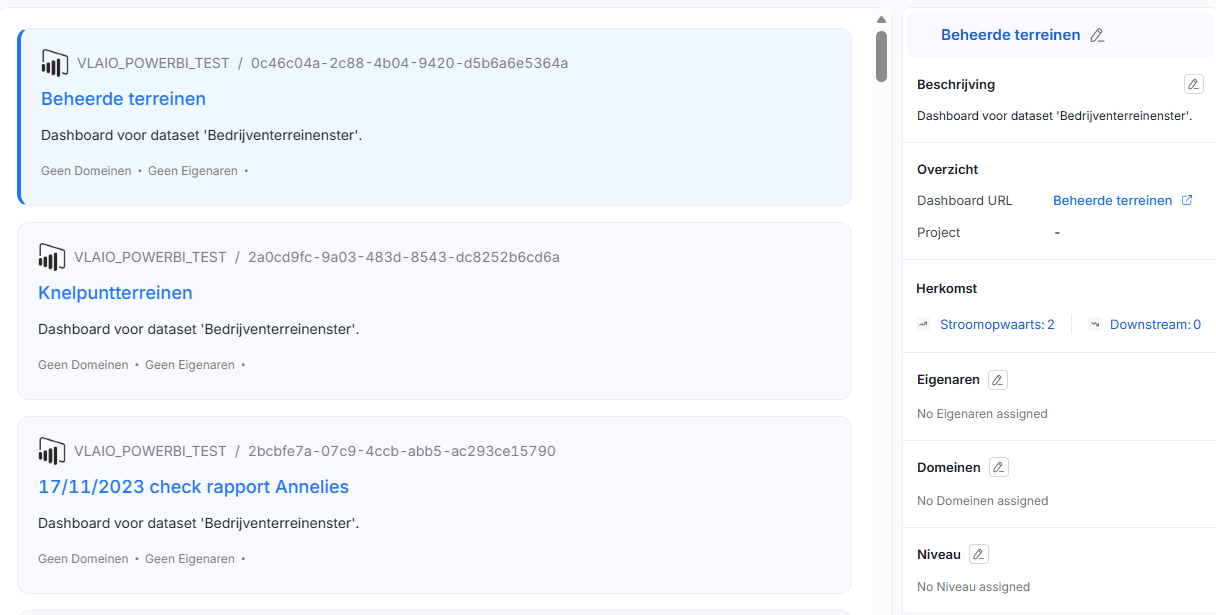
\includegraphics[width=\textwidth]{images/om-dashboard.png}
	\caption{OpenMetadata Dashboard}
	\label{fig:openmetadata-dashboard}
\end{figure}

De toegevoegde waarde van deze PoC uit zich in de praktijk via twee concrete scenario's, namelijk het traceren van de herkomst vanaf een specifiek rapport en het inschatten van de impact vanaf een centrale dataset.\\

Ten eerste maakt het platform het mogelijk om vanuit de bu\-si\-ness-om\-ge\-ving terug te redeneren naar de bron (upstream lineage). Wanneer een eindgebruiker twijfelt over de data in een specifiek dashboard, kan via de gebruikersinterface van OpenMetadata gemakkelijk worden gecontroleerd welke platinum-dataset de bron vormt. Op Figuur~\ref{fig:lineage_bedrijvents_rep} en Figuur~\ref{fig:lineage_kris_rep} is dit zichtbaar. Dit lost de `zichtbaarheidskloof' op dat besproken werd in vorig hoofdstuk. Een moet dus niet langer in de Power BI-instellingen of Databricks-notebooks zoeken naar de achterliggende databron.\\

\begin{figure}[H]
	\centering
	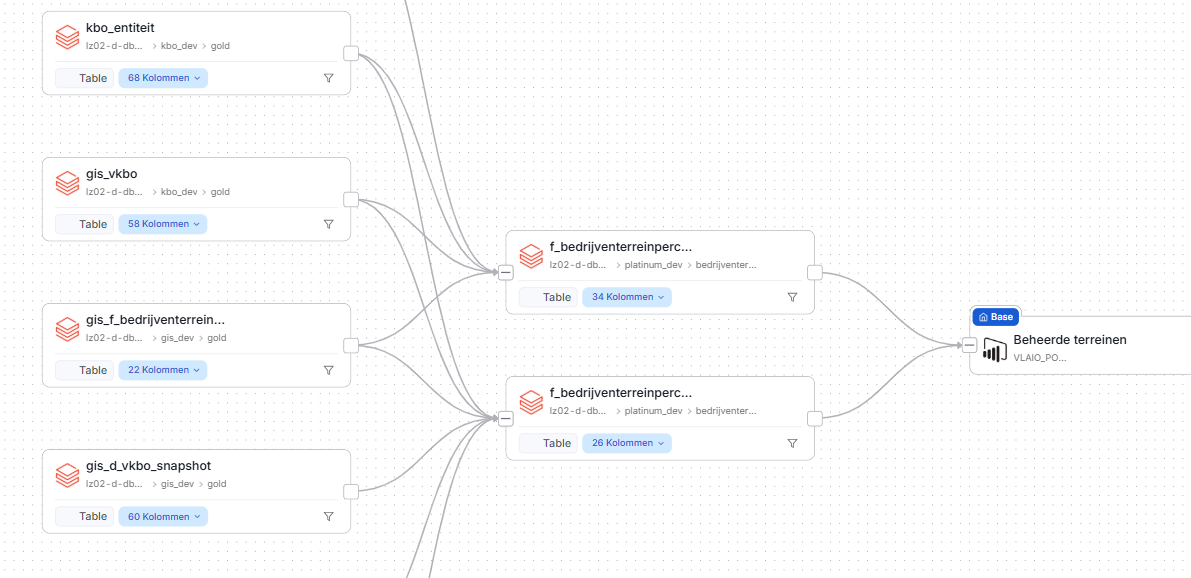
\includegraphics[width=0.9\textwidth]{images/rapport_bedrijven.png}
	\caption{Upstream lineage bedrijventerreinster}
	\label{fig:lineage_bedrijvents_rep}
\end{figure}

\begin{figure}[H]
	\centering
	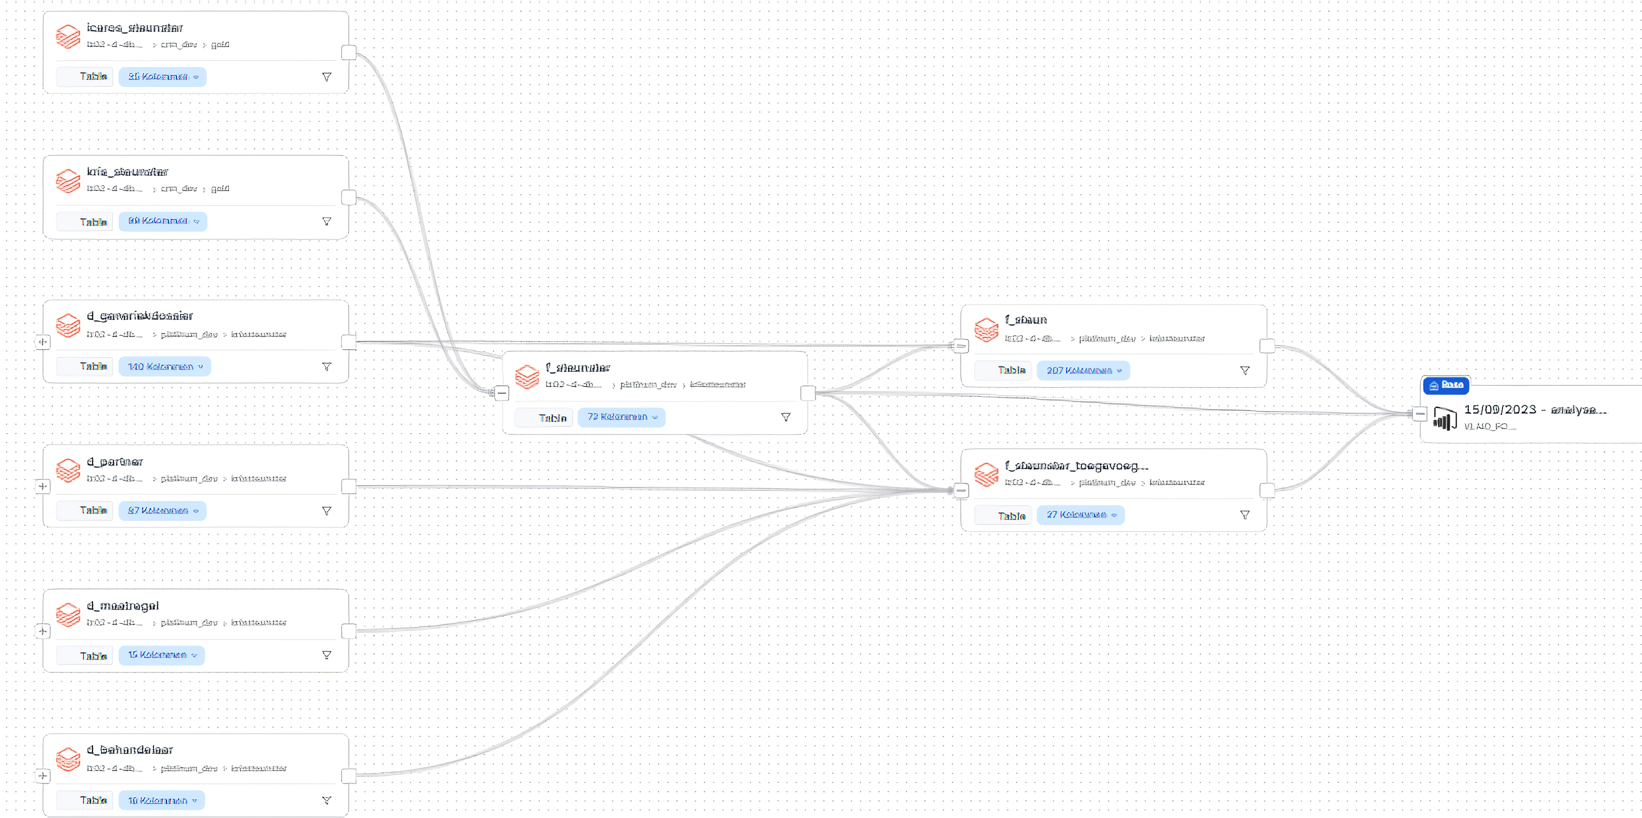
\includegraphics[width=0.9\textwidth]{images/rapport_krissteunster.png}
	\caption{Upstream lineage krissteunster}
	\label{fig:lineage_kris_rep}
\end{figure}

Het tweede scenario draait om impactanalyse vanuit het perspectief van databeheer (downstream lineage). Voor data-engineers of beheerders is het cruciaal om te weten wat de gevolgen zijn als een tabel in de platinum-laag of een onderliggende laag gewijzigd wordt. Figuur~\ref{fig:lineage_dataset_impact} illustreert hoe de nieuwe metadata integreert in het grotere geheel. De figuur toont niet alleen de reeds bestaande database-views, maar ook de volledige set Power BI-rapporten die via deze PoC aan de centrale \texttt{steunster}-tabel zijn gekoppeld. Mocht er in de toekomst iets veranderen aan de structuur van deze platinum-dataset of een onderliggende dataset, dan is direct duidelijk welke rapporten risico lopen en welke business-eigenaren dus geinformeerd moeten worden.\\

\begin{figure}[H]
	\centering
	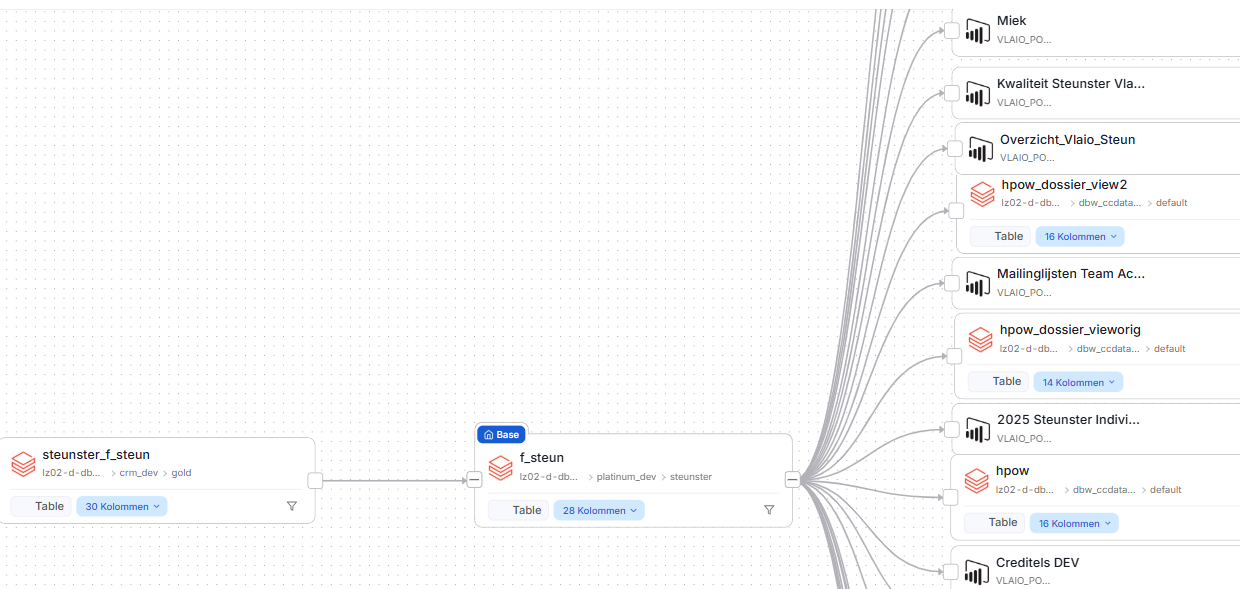
\includegraphics[width=0.9\textwidth]{images/dataset_steunster_impact.png}
	\caption{Downstream lineage: alle gekoppelde Power BI-rapporten een dataset.}
	\label{fig:lineage_dataset_impact}
\end{figure}
